%%%%%%%%%%%%%%%%%%%%%%%%%%%%%%%%%%%%%%%%%%%%%%%%%%%%%%%%%%%%%%%%%%%%%%%%%%%
\chapter{Review of Related Systems and Related Literature}
%%%%%%%%%%%%%%%%%%%%%%%%%%%%%%%%%%%%%%%%%%%%%%%%%%%%%%%%%%%%%%%%%%%%%%%%%%%
		Machine-assisted parsing of journal citations encounters problems apparent in all textual retrieval tasks in mass applied media. The variations in official citation styles, the deviations within an official citation styles and same authors and journals written in different ways are but the first difficulties in the road for complete machine-assisted citation parsing.

	However, there have been previous works on citation parsing, complete with online, public citation parsers with API. Much like this study, these parsers merely parse through the data inputted. They do not process the rank, nor perform image-processing data extraction. Two of the most widely used citation parsers found online are FreeCite and ParsCit.

\section{FreeCite and ParsCit}
FreeCite is an open-sourced application that parses through the citations of various documentations into fielded data. It can be freely used as an application or service, under MIT license. FreeCite was developed by the Brown University in partnership with Public Display, a Providence-based start-up company, in inspiration to ParsCit \cite{freecite}.

	ParsCit primarily performs two tasks, the reference of string parsing, may it be citation parsing and citation extraction, and logical structure parsing of documents. Its architecture is that of a supervised machine-learning system that utilizes Conditional Random Fields as its learning mechanism. \cite{parscit}. Like FreeCite, the software is licensed in such a way (Lesser GNU Public License) that the public is free to utilize it in their own projects.

These parsers function to extract the data to make citation based ranking easier. In measuring citation impact, different measures may be employed although a naive way to do this is through its citation count \cite{citation_frequency}. Often times, the more citations a journal has, it can then be said that it is more "central" \cite{eigenfactor_rank}. However, merely counting citations of a particular article is ineffective. In the identification of citations for proper parsing, certain conditions must be analyzed and accounted for.

\section{Identity Uncertainty}
Identity uncertainty is a prevalent and unavoidable problem in citation matching. This phenomenon occurs if identifiers are absent in token sequences which may result in ambiguous observations for certain objects. This problem is addressed by constructing Relational Probability Models (RPMs) which consist of attributes that a citation may contain. RPMs semantics assume that unique names exist for different papers (although they may be the same) unless proven otherwise. Uniqueness is decided by the mapping which has the least co-referring terms. The RPMs can then be expressed to an equivalent Bayesian network where attributes of the objects are constructed as nodes. If citation C1 and C2 correspond to the paper P1 and P2 where P1 and P2 are the same object, the models will share one set of the same attributes \cite{identity_uncert}. A Markov Chain Monte Carlo based algorithm is then used to match the citations. \cite{markov}

\begin{figure}[H]
    \centering
    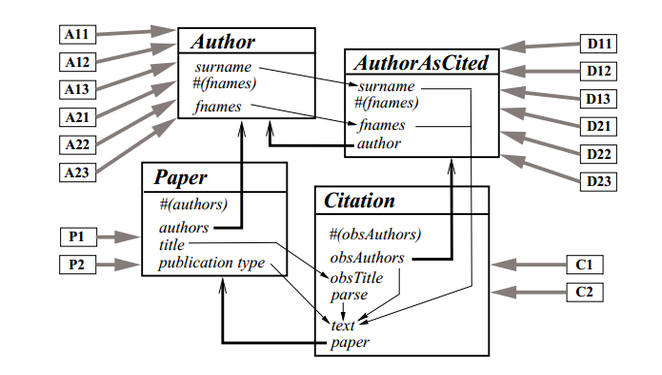
\includegraphics[width=0.8\textwidth]{RPM.png}
    \caption{Relational Probability Model}
    \label{fig:RPM}
\end{figure}

The image above serves as an example of  Citeseer. The large rectangles represent classes: the dark arrows indicate the ranges of their complex attributes, and the light arrows lay out all the probabilistic dependencies of their basic attributes. The small rectangles represent instances, linked to their classes with thick grey arrows. We omit the instance statements which set many of the complex attributes.

\section{Data Catching and Citation Parsing}

		In order to extract the necessary information, a parser is required to sift through the text and separate the necessary from the unnecessary. The problem of citation extraction is the segmentation of oftentimes unstructured or ill-structured citations into proper segments, where data and its classification can be properly identified. Several methods have been proposed in the recent years for the extraction of data from textual documents. The methods can be generally defined into two categories: knowledge-based approach, and learning -based approach. \cite{bibpro}

	The knowledge-based approach derives ontology that describes the data of interest using domain knowledge, where the knowledge includes relationships, lexical appearances and context keywords. From the parsing the ontology, several rules and an extractor can be generated, which is then used to extract the data. This particular method is more widely used in real-world applications, with a well-known example on CiteSeer. CiteSeer is a popular search engine and digital library that extracts metadata from citations using heuristics, with an identification accuracy of titles and authors at 80% and page number accuracy of 40% \cite{citeseer}.  However, the database that CiteSeer’s system relies on must be maintained by a domain expert, making the presence of such an expert necessary.

	Other applications of knowledge-based approach are CRAM \cite{cram}, FLUX-CiM \cite{flux}, and INFOMAP \cite{infmap}. CRAM develops an automatic segmentation system for its inputs by mining tables in relational databases and data warehouses. FLUX-CiM can automatically create ontology for a given area, constructed from an existing set of sample metadata records.  The FLUX-SiM dataset, its own set of reference data to be used for testing and benchmarking, contains citations from two domains, Computer Science and Health Science. INFOMAP relies on a tree-based representation scheme that organizes reference concepts in a hierarchical manner. For the six major citation formats, it has an overall average of 92.39% \cite{bibpro}. The INFOMAP dataset has roughly 160,000 citations records in 6 different citation styles.

	The learning-based approach focuses on the classification of the citation data in question, using machine learning in order to solve it. This requires training data in order to function properly, slightly similar to the FLUX-CiM stated above. Currently, there are three major machine learning techniques, the Support Vector Machines \cite{svm}, Hidden Markov Model \cite{markov}, and Conditional Random Fields \cite{crf}.  They are used to extract information from research papers and journal articles, and has shown great performance to the Cora dataset. The Cora dataset is the most widely used benchmarking dataset for machine learning techniques \cite{cora}. 

This particular method has great adaptability, mainly due to its nature as a machine-learning method. However, it does possess some limitations. The quality of training data directly affects the performance of the method \cite{bibpro}. A faulty set of training data can render the entire process useless. 

	This machine-assisted process that this thesis will focus on shall be under knowledge-based approach. This method allows for the use of keywords and lexicons, without relying on the creation of proper training data. 
